\section{Design of the LNA}

In this section, we present the design of the LNA architecture shown in Figure \ref{fig:schem-lna}. The design process involves biasing conditions and ensuring the desired specifications are met.

\textcolor{red}{Dizer objetivos zin = 50, largura de banda ganho e noise E xplicar a cenas das capacitancias}
\label{sec:inpCap}
Input Capacitances will be a problem especially for the smaller nodes, where the band is higher frequencies. 
\textcolor{red}{Explicar "workflow" valores teoricos com o script -> .op -> e ajustar para o resto dos valores}

\textcolor{red}{Dizer que inicialmente gds << gm e gmbb = 0.2 gm, e para gds depois do primeiro valor o valor de gds ]e atualizado e valores sao retirados outra vez, e de resto os valores sao usados para fine tuning. Explicar o valor de vdssat e zonas de funcionameto do transistor}

It is important to note that the value of $r_{ds}$ is hard to calculate, and therefore a first biasing circuit is simulated and the circuit is recalculated with the new value of rds.

Vdsat inicial
$V_{DSsat} = \SI{100}{\milli\volt}$

\begin{equation}
    g_{mb}\approx 0.2\cdot g_m
    \label{eq:gmb_approx}
\end{equation}
$g_{ds}\propto \frac{L}{I_D}$\cite{AnalogCircDesign}

\begin{equation}
    g_m =\sqrt{2K_{n,p}\frac{W}{L}I_D}= \frac{2I_D}{V_{DSsat}}
    \text{\cite{AnalogCircDesign}}
    \label{eq:gm_eq}
\end{equation}

\begin{equation}
    I_D=\frac{K_n}{2}\cdot\frac{W}{L}V_{DSsat}^2
    \text{\cite{AnalogCircDesign}}
    \label{eq:ID_eq}
\end{equation}

\textcolor{red}{Falta falar do ganho}


\subsection{Common Gate Stage Design}


\begin{figure}[h]
    \centering
    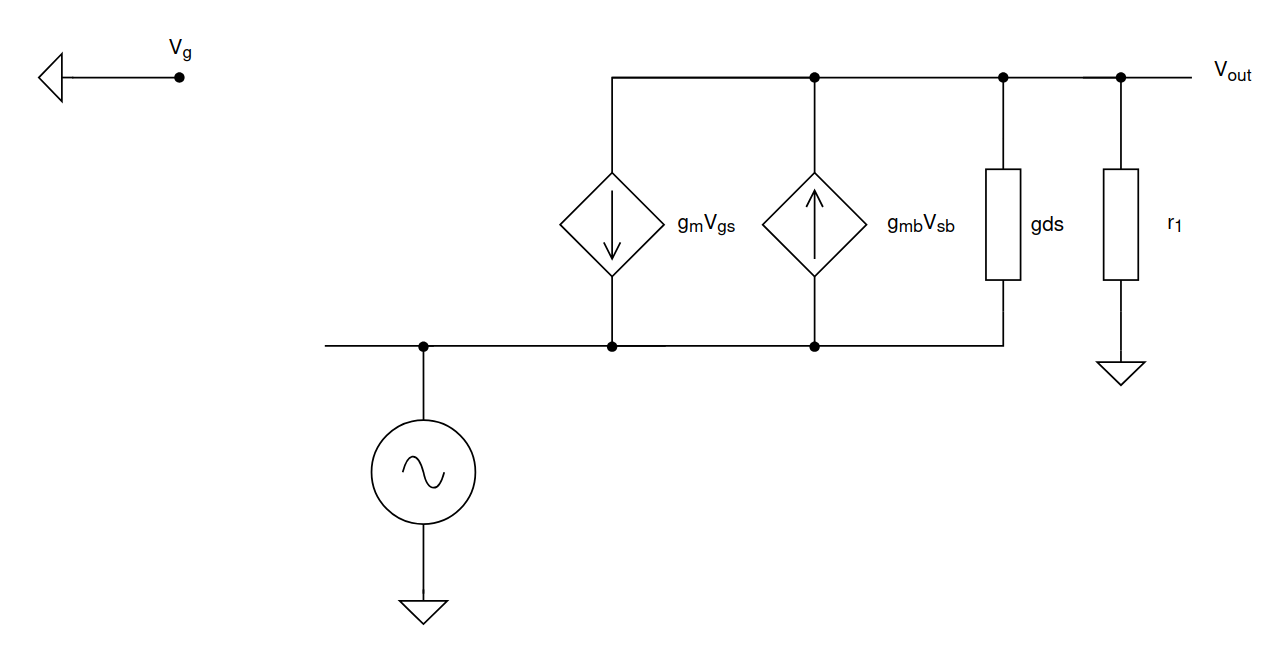
\includegraphics[width=1\textwidth]{Images/CG_SmallSignal.png}
    \caption{Common Gate Small Signal Schematic.}
    \label{fig:CG_SmallSignal}
\end{figure}

\begin{equation}
    A_v = \frac{v_o}{v_i}=\frac{g_m+g_{mb}+g_{ds}}{g_{ds}+1/r_1}
    \label{eq:CSGain}
\end{equation}

\begin{equation}
    Z_{in} = \frac{V_i}{I_i}=\frac{1}{- \frac{g_{ds} \left(g_{ds} + \frac{1}{r_{1}}\right)}{g_{ds} + g_{m} + g_{mb}} + g_{ds} + g_{m} + g_{mb}}\approx\frac{1}{g_m+g_{mb}}
    \label{eq:CG_Zin}
\end{equation}

\subsubsection{Circuit sizing}

Using approximation presented in Equation \ref{eq:gmb_approx}, in order to meet the $Z_{in}$ specification $g_m \approx \SI{16.7}{\milli\siemens}$.

Knowing this, from Equation \ref{eq:gm_eq} and with the inicial value of $V_{DSsat}$, $I_D$ is calculated.

Then it is possible to get the value of $W/L$, using Equation \ref{eq:gm_eq}.

Finally to meet the Gain specification, analyzing Equation \ref{eq:CSGain}, it will only depend on the $r_1$ value. 

In this stage, $I_D$ is forced by a current source, therefore, $V_{DSsat}$ will be fixed, hence, $V_{bias}$ needs only to be high enough so that $V_{s }> 0$ but not so high that $V_s > V_d$, $V_d = V_{dd} - r_1\cdot I_D$. 

\subsection{Common Source Stage Design}


\begin{figure}[H]
    \centering
    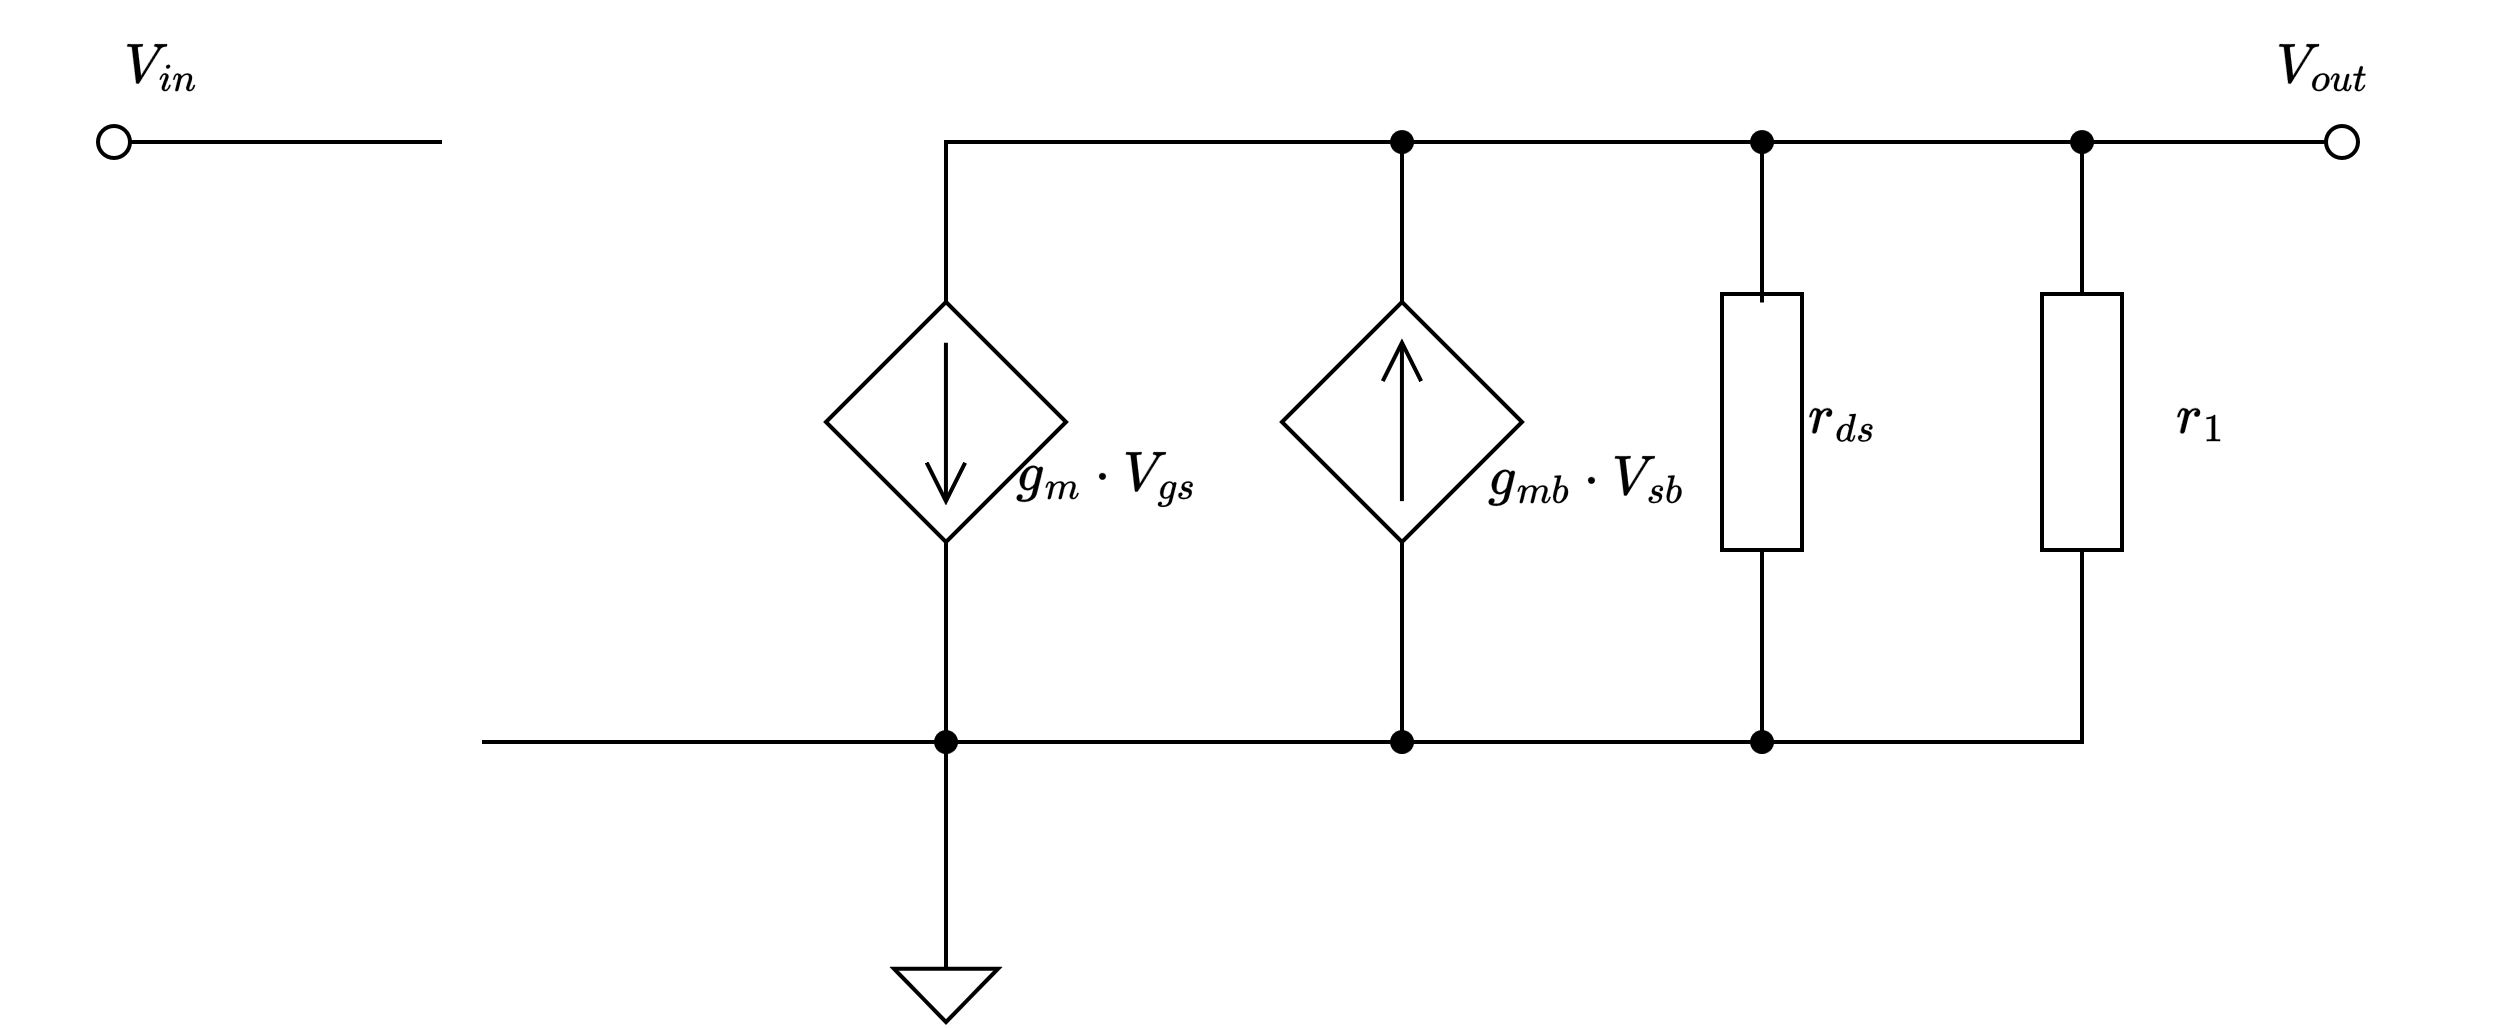
\includegraphics[width=1\textwidth]{Images/CS_SmallSig.png}
    \caption{Common Source Small Signal Schematic.}
    \label{fig:CS_SmallSignal}
\end{figure}

\begin{equation}
    A_v = -gm(rds//R_L)
    \label{eq:CS_Gain}
\end{equation}

\begin{equation}
    Z_{in} \approx +\infty
    \label{eq:CS_Zin}
\end{equation}

\subsubsection{Circuit Sizing}

For the Common Source $Z_{in}$ is not important, although the input capacitances will have a great effect on the circuit performance has explained in section \ref{sec:inpCap}. 

There are already fixed parameters, $V_{DSsat}$, in order to garante the device is in the active zone, and $g_{m}$ will have two distinct values at first it will be the same as the Common-Gate, and at a second phase it will 3 times larger. 

With the fixed values , using Equation \ref{eq:gm_eq}, $W/L$ is obtained, Equation \ref{eq:wl2}. 

\begin{equation}
    \begin{split}
        g_{m_1} &= n\cdot g_{m_2} = K_{n}\frac{W}{L}V_{DSsat}\text{\cite{AnalogCircDesign}} \Leftrightarrow \\
       \Leftrightarrow \frac{W}{L} &= \frac{g_{m2}}{K_n \cdot V_{DSsat}^2}
    \end{split}
    \label{eq:wl2}
\end{equation}

The value of $r_2$ can be also calculated as a function the gain goal, Equation \ref{eq:r2}. 

\begin{equation}
    \begin{split}
        r_{2} = - \frac{A_{v} r_{ds}}{A_{v} - g_{m} r_{ds}}
    \end{split}
    \label{eq:r2}
\end{equation}


\subsubsection{$V_{bias}$ Sizing}


In this stage $V_{bias}$ is a straight forward calculating, since $V_{gs} = V_{bias}$.

\subsubsection{n Factor effect on $g_m$}

\subsection{Buffer Stage Design}